\documentclass[11pt]{article}

\usepackage[letterpaper,margin=0.75in]{geometry}
\usepackage{graphicx}
\usepackage{listings}
\usepackage{subfigure}

\begin{document}

\title{Lab \#1 Report}

\author{Tyler Southwick, Taylor Southwick}

\date{}

\maketitle

\section{Potential Fields}
\subsection{four\_ls}

\begin{figure}[h!]
	\caption{Potential field towards flag or base}
	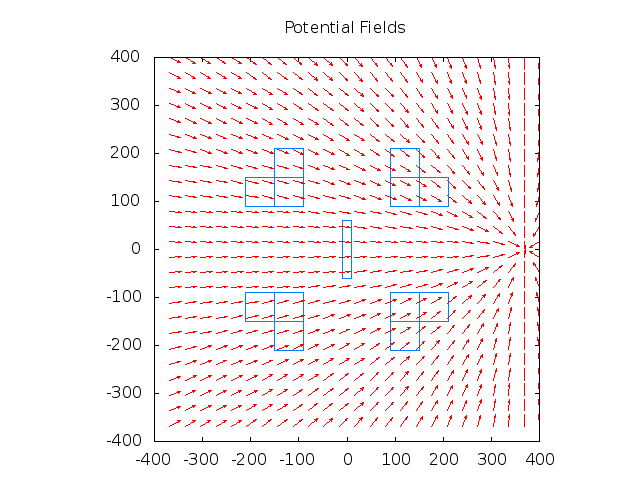
\includegraphics[scale=.4]{plots/four_ls/pfFlag.png}
\end{figure}
\begin{figure}[h!]
	\caption{Potential fields away from obstacles}
	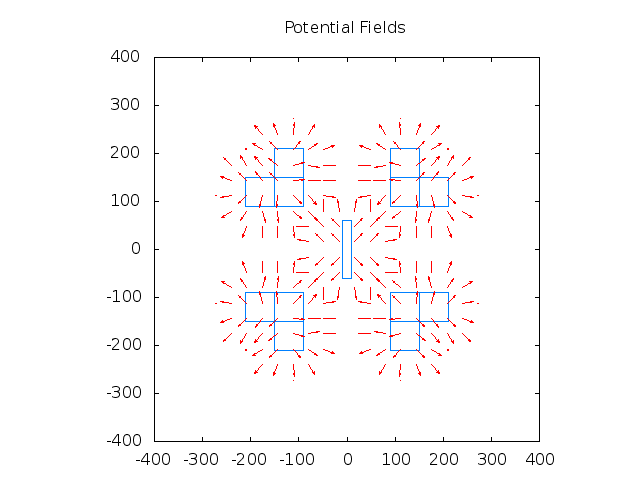
\includegraphics[scale=.4]{plots/four_ls/pfObstacles.png}
\end{figure}
\begin{figure}[h!]
	\caption{Potential field towards flag or base and away from obstacles}
	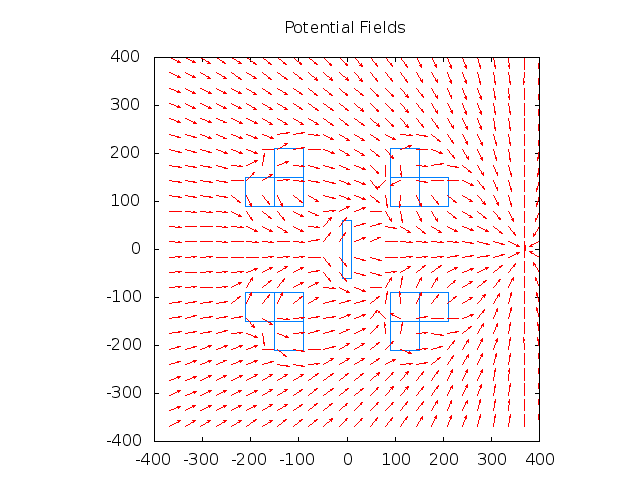
\includegraphics[scale=.4]{plots/four_ls/pfFlagsAndObstacles.png}
\end{figure}

\subsection{rotated squares}

\begin{figure}[h!]
	\caption{Potential field towards flag or base}
	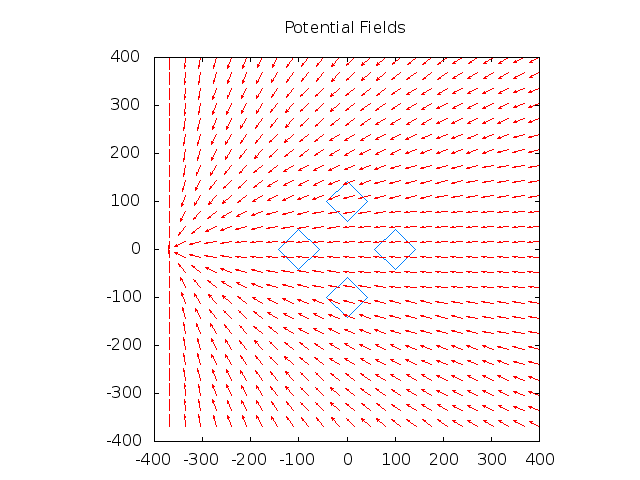
\includegraphics[scale=.4]{plots/rotated_box_world/pfFlag.png}
\end{figure}
\begin{figure}[h!]
	\caption{Potential fields away from obstacles}
	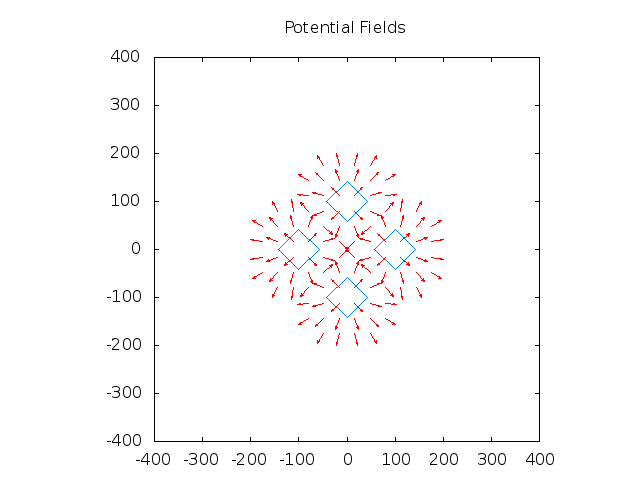
\includegraphics[scale=.4]{plots/rotated_box_world/pfObstacles.png}
\end{figure}
\begin{figure}[h!]
	\caption{Potential field towards flag or base and away from obstacles}
	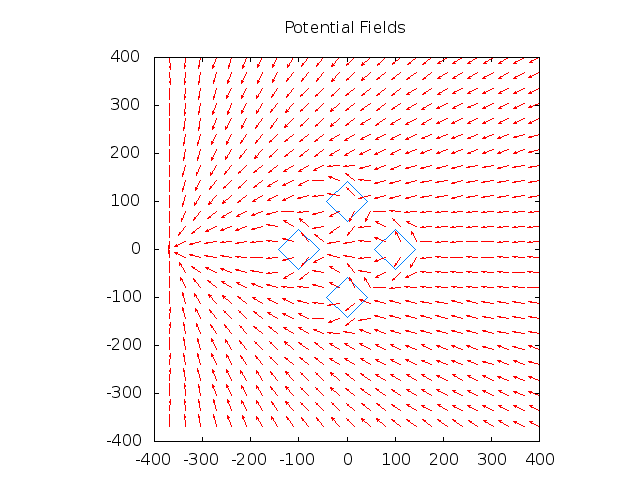
\includegraphics[scale=.4]{plots/rotated_box_world/pfFlagsAndObstacles.png}
\end{figure}

\end{document}
